\section{Analyzing the system and it's architecture}
The architecture of the system is important because it dictates the means by which scalability can be obtained. In Fig. \ref{fig:systemArchitecture} the architecture of the system is presented, this architecture being an extension of [cite paper from SYNASC]. The system is composed of 7 components: FrontEnd, Scanner, Converter, Presenter, Remediator, a document database and a message queue. The first five components send messages using the queue and are completely decoupled from one another, from each component perspective the system is only compose of itself and one or more message queues. This decoupling provides grate opportunity for replication and scalability.

\begin{figure}[ht]
\centering
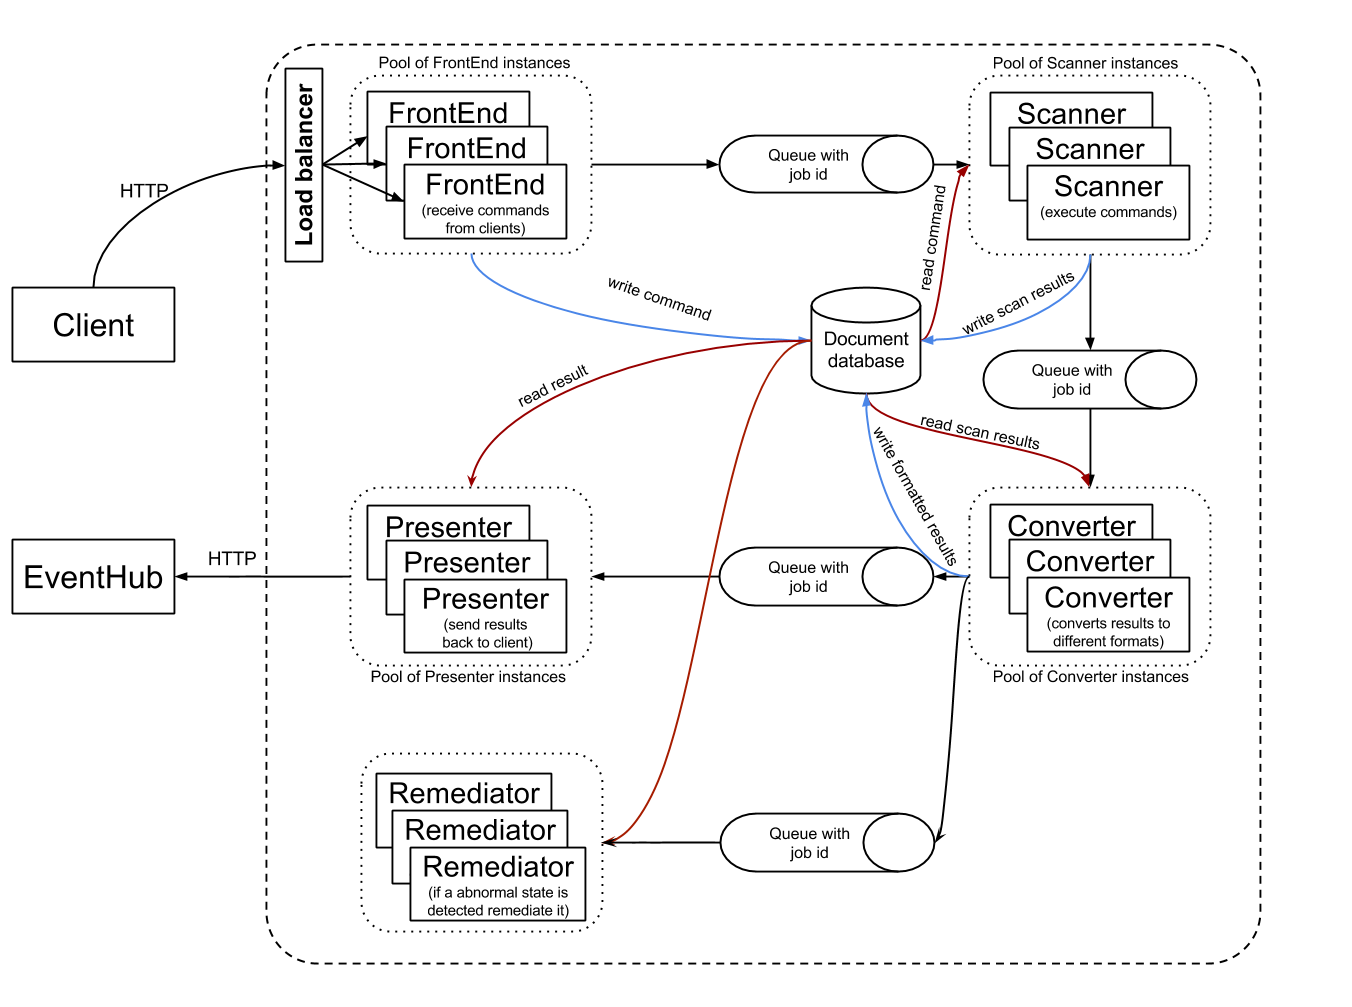
\includegraphics[width=\linewidth]{./img/MonitoringSystemArchitectureRemediation.png}
\caption{Distributed monitoring system architecture}
\label{fig:systemArchitecture}
\end{figure}

